\begin{figure*}[htbp]
	\centering
	\includegraphics[width=\linewidth]{img/net/net}
	\caption{The cycle regularization implemented along with networks: (a) is the implementation with AtlasNet\cite{atlasnet}. $f$ is the forward 3D surface decoder in original network and $g$ is our inverse decoder used to form the regularization term. (b) is the implementation with Pixel2Mesh\cite{pixel2mesh}.  Pixel2Mesh\cite{pixel2mesh} adopt the coarse-to-fine framework and use three \emph{G-ResNet} block ($f_1,f_2,f_3$) to map the mesh to target shape on three different point density. The \emph{Graph -Unpooling} layers are used to do the upsampling. In other words, they upsample $Y_1$ to $X_2$ and $Y_2$ to $X_3$ base on connected graph in mesh. We use three point-wise MLP ($g_1,g_2,g_3$) as inverse decoders for each level of point density and form a regularization term for each level.}
	\label{fig:net}
\end{figure*}
\section{Method}
In this section, we firstly show that the we can make sure that there is no overlapped points on target surface by enforcing the mapping to be injective. 
Then we propose the cycle regularization technique and explain in details (as shown in Figure~\ref{fig:net}) about how we respectively apply this general technique onto AtlasNet\cite{atlasnet} and Pixel2Mesh\cite{pixel2mesh}, whose network structures are quite different from each other. 
\subsection{Injective mapping and self-overlapped points}
\label{subsec:inj}
Start with the definition of injective mapping at \textbf{Definition}~\ref{def:injective}, we can intuitively induce the conclusion that given a predefined surface with $ X =\{\mathbf{x}~|~\mathbf{x}$ is a point on the predefined surface $ \} $, a target surface with $ Y =\{\mathbf{y}~|~\mathbf{y}$ is a point on the target surface $ \} $ and a function $f:X \rightarrow Y$. If $\exists$ $ \mathbf{a},\mathbf{b} \in X$, $\mathbf{a} \neq \mathbf{b}$ and $f(\mathbf{a}) = f(\mathbf{b})$ (i.e. the overlapped points on target surface exists) then by definition, $f$ is not an injective function. Equivalently (as the converse negative proposition), we can make sure there is no self-overlapped points on the target surface by enforcing $f$ to be injective.
\begin{m_def}
\label{def:injective}
Let $f$ be a function whose domain is a set $X$. The function $f$ is said to be injective provided that
\begin{equation}
\forall a,b \in X, f(a) = f(b) \Rightarrow a = b.
\end{equation}
Equivalently, 
\begin{equation}
\forall a,b \in X, a \neq b \Rightarrow f(a) \neq f(b).
\end{equation}
\end{m_def}

\subsection{Cycle regularization}
\label{subsec:cyclereg}
\begin{m_thm}
\label{thm:injective}
functions with left inverses are always injective. That is, given $f:X \rightarrow Y$, if there is a function $g:Y \rightarrow X$ such that,
\begin{equation}
\label{equ:injective}
\forall x \in X,~g(f(x)) = x,
\end{equation}
then $f$ is injective.
\end{m_thm}

Based on \textbf{Theorem}~\ref{thm:injective}, we turn an injective constraint to our cycle regularization term as:
\begin{equation}
\label{equ:cycle_term}
cycle_X(f)=\min_g\sum_{\mathbf{x}\in X}||g(f(\mathbf{x})) - \mathbf{x}||_2^2.
\end{equation}
By minimizing this term to zero:
\begin{equation}
f^* = \arg\min_f cycle_X(f)
\end{equation}
we can get the $f^*$ that has the left inverse function $g$, therefore $f^*$ is injective. 

However, it is never possible to actually minimize a regularization term to zero, especially in training neural networks. But when this term is minimized to sufficiently small then we can construct $g^*$ based on $g$ that is the left inverse function of $f^*$ and guarantee that $f^*$ is injective. A very tight example is that when the regularization term is so small that $g(f(\mathbf{x}))$ is closer to $\mathbf{x}$ than any other point in $X$. Such example can be summarized by \textbf{Proposition}~\ref{prop:nearest}.

\begin{m_prop}
	\label{prop:nearest}
	Given sets $X$ and $Y$ that are subset of Euclidean space $\mathcal{R}^3$, function $f:X \rightarrow Y$  and function $g:Y \rightarrow X$, if
	\begin{equation}
	\exists~g, \max_{\mathbf{x}\in X}|| g(f(\mathbf{x})) - \mathbf{x} ||_2^2 < \min_{\mathbf{a},\mathbf{b} \in X}|| \mathbf{a} - \mathbf{b} ||_2^2,
	\end{equation}
	then $f$ is injective.
\end{m_prop}

\textbf{Proposition}~\ref{prop:nearest} can be proved by simplely composite nearest neighbor with the function $g$. We can construct nearest neighbor function $l: \mathcal{R}^3 \rightarrow X $ as:
\begin{equation}
\forall \mathbf{a} \in \mathcal{R}^3, l(\mathbf{a}) = \arg\min_{\mathbf{b} \in X} || \mathbf{a} - \mathbf{b} ||_2^2
\end{equation}
then
\begin{equation}
\begin{aligned}
&\max_{\mathbf{x}\in X}|| g(f(\mathbf{x})) - \mathbf{x} ||_2^2 < \min_{\mathbf{a},\mathbf{b} \in X}|| \mathbf{a} - \mathbf{b} ||_2^2\\
&\Rightarrow || g(f(\mathbf{x})) - \mathbf{x} ||_2^2 \leq \min_{\mathbf{a},\mathbf{b} \in X}|| \mathbf{a} - \mathbf{b} ||_2^2\\
&\Rightarrow || g(f(\mathbf{x})) - \mathbf{x} ||_2^2 \leq \min_{\mathbf{b} \in X}|| g(f(\mathbf{x})) - \mathbf{b} ||_2^2\\
&\Rightarrow l(g(f(\mathbf{x}))) = \mathbf{x}\\
\end{aligned}
\end{equation}
then $g^*(\mathbf{y}) = l(g(\mathbf{y}))$ is the left inverse of $f$, therefore $f$ is injective.

\noindent\textbf{Remaining gap}
Even when the condition in Proposition~\ref{prop:nearest} is met after optimization, there is still no guarantee for $f$ being injective over the continue surface. The reason is that when we turn Equ.~(\ref{equ:injective}) into Equ.~(\ref{equ:cycle_term}), we actually change the constraint over continue surface into term defined on discrete point set. We believe that if $f$ and $g$ are linearly extended to entire continue surface, then being injective may be better extended to continue surface, since we are using triangle meshes and we can establish bijective mapping between two triangles by linear interpolation. This is why we use point-wise MLP and ReLU activations as our inverse decoder $g$.
\begin{figure*}[htbp]
	\centering
	\includegraphics[width=\linewidth]{img/opt/opt}
	\caption{Visualize convergence of optimization: When optimized with our cycle regularization term, the term take effect after only few iterations. It not only keep the mapping injective in optimization but also correct the self-intersection from the initialization. When optimized without cycle regularization term, the surface usually converge to a surface with self-intersection.}
	\label{fig:opt}
\end{figure*}


\subsection{Implementation along with networks}

As stated in AtlasNet\cite{atlasnet}, it is possible to use multilayer perceptron with ReLU nonlinearities and enough hidden units to approximate any shape within a small positive error $\epsilon$. In practice, we employ another 3D surface decoder to approximate $g$. Then we explain how we implement this technique for AtlasNet and Pixel2Mesh respectively. Generally speaking, we reuse the network structures from their network respectively and show that our cycle regularization is a general technique for this type of networks.

\noindent\textbf{AtlasNet} Depending on a shape representing feature $\mathbf{s}$, the AtlasNet use point-wise MLP
$f$ with parameters $\theta_f$ to learn to map points in $X=\{\mathbf{x}| \mathbf{x}$ are points uniformally sampled from predefined surface $P\}$ to points in $Y=\{\mathbf{y}| \mathbf{y}$ are points uniformally sampled from surface $S\}$. In implementation, $P$ can be either unit square $[0,1]^2$ or the surface of a 3D sphere. $S$ is the target surface, which is usually the surface of an object in AtlasNet\cite{atlasnet} and in this paper. Then we use another point-wise MLP $g$ with parameters $\theta_g$ to map points from $Y$ back to $X$. Along with our cycle regularization  total loss function for AtlasNet can be written as:

\begin{figure*}[htbp]
	\centering
	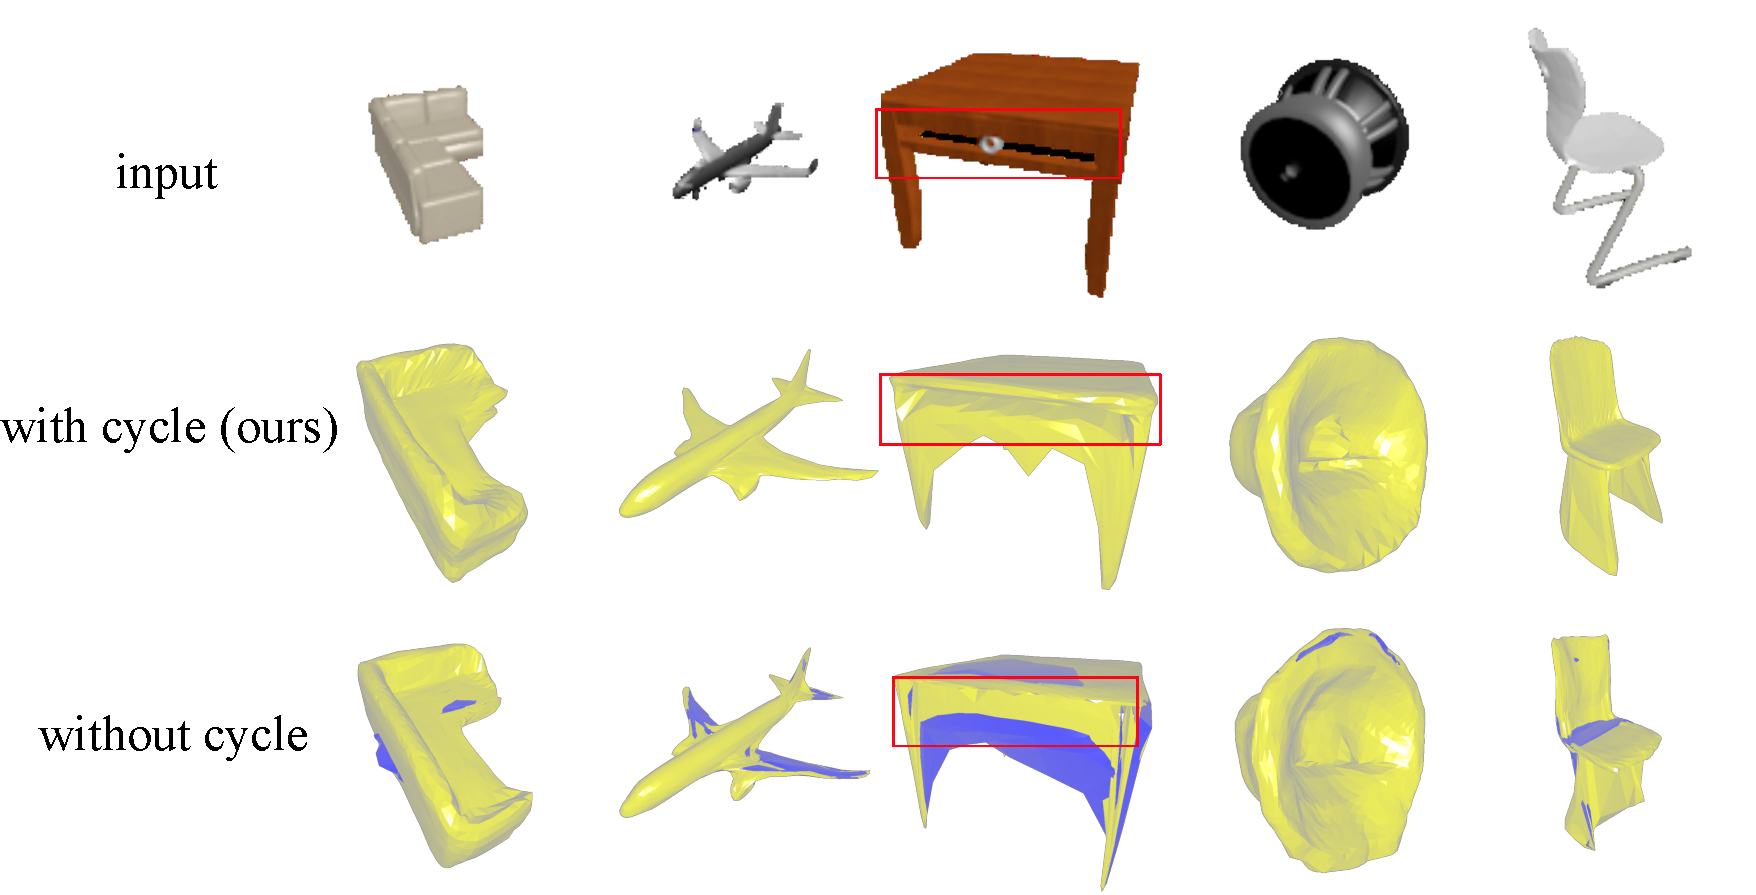
\includegraphics[width=\linewidth]{img/atlas/svr}
	\caption{Cycle regularization on AtlasNet: All the visualized cases here are selected from the test set of AtlasNet. Some meshes' view direction are manually adjusted to better expose the differences. The red rectangles are highlighting a case (the table) in which more details are preserved than the original network because we are enforcing the surface to be free of self-intersection with our cycle regularization term}
	\label{fig:svr}
\end{figure*}

\begin{equation}
\begin{aligned}
\label{equ:atlascycle}
\mathcal{L}_{(X,Y)}(\theta_f,\theta_g) &= \sum_{\mathbf{x} \in X} \min_{\mathbf{y} \in Y}|| f_{\theta_f}(\mathbf{x};\mathbf{s}) - \mathbf{y} ||_2^2 \\ &+ \sum_{ \mathbf{y} \in Y}\min_{ \mathbf{x} \in X} || f_{\theta_f}(\mathbf{x};\mathbf{s}) - \mathbf{y} ||_2^2 \\ &+ \lambda\sum_{\mathbf{x} \in X}||g_{\theta_g}(f_{\theta_f}(\mathbf{x};\mathbf{s});\mathbf{s}) - \mathbf{x}||_2^2,
\end{aligned}
 \end{equation}
In which, the shape representation feature is simply concatenated to each point so that the $f$ and $g$ is depending on a global shape representing feature $\mathbf{s}$. $\lambda$ is the weight for cycle regularization. In AtlasNet, $\mathbf{s}$ is generated from either PointNet\cite{resnet} for auto-encoding or ResNet-18\cite{resnet} for single view reconstruction. In implementation $g$ is a MLP with same number of units in hidden layers as $f$, as shown in Figure~\ref{fig:net}.

\noindent\textbf{Pixel2Mesh}
Comparing to AtlasNet, the Pixel2Mesh\cite{pixel2mesh} use a more complicate network structure. In order to implement cycle regularization along with Pixel2Mesh, we need to cope with two features in the network of Pixel2Mesh. 
One is the coarse-to-fine framework adopted by Pixel2Mesh. It uses three blocks of graph based convolution residual network ($f_1,f_2,f_3$ shown in Figure~\ref{fig:net}) to map mesh based features to target surface at three different level of point density. To be compatible with such framework, we also use three point-wise MLP as inverse decoder and form our regularization term as:
\begin{equation}
\begin{aligned}
\mathcal{L}_{cycle}(\theta_f,\theta_g) &= \sum_{\mathbf{x} \in X_1}||g_{1}(f_{1}(\mathbf{s}_1,\mathbf{x})) - \mathbf{x}||_2^2\\
&+ \sum_{\mathbf{x} \in X_2}||g_{2}(f_{2}(\mathbf{s}_2,\mathbf{x})) - \mathbf{x}||_2^2\\
&+ \sum_{\mathbf{x} \in X_3}||g_{3}(f_{3}(\mathbf{s}_3,\mathbf{x})) - \mathbf{x}||_2^2,
\end{aligned}
\end{equation}
in which, $\theta_f$ is the whole parameters for $f_1,f_2,f_3$. $\theta_g$ is the whole parameters for $g_1,g_2,g_3$. $\mathbf{s}_1,\mathbf{s}_2,\mathbf{s}_3$ are features extracted from different layers of VGG-16 based on input point positions $X_1,X_2,X_3$ in original network. We add our regularization term to original loss function of Pixel2Mesh with a weight $\lambda$. (Please refer to Pixel2Mesh\cite{pixel2mesh} for more details of the entire loss function)

The other feature we need to cope with is that Pixel2Mesh is based on the graph convolution framework from \cite{graphconv}. In its implementation the supports are not continuously stored, they are inputed as sparse indexes, which makes the implementation of point-wise MLP different from conventional ones. However, it is still quite simple to do so, since the Pixel2Mesh already implemented the graph convolution layer as:
\begin{equation}
\mathbf{y}_p^{(l+1)} = w_0 \mathbf{y}_p^l + \sum_{q\in\mathcal{N}(p)} w_1\mathbf{y}_q^l + \mathbf{b},
\end{equation}
in which,  $\mathbf{y}_p^l$ is the feature vector $\mathbf{y}$ at support $p$ (corresponding to a vertex on mesh) of layer $l$. $q\in N(p)$ means that $q$ is neighbor support of $p$ in graph. We can implement point-wise MLP by removing neighbor related term as:
\begin{equation}
\mathbf{y}_p^{(l+1)} = w_0 \mathbf{y}_p^l + \mathbf{b},
\end{equation}
For more details, please go to our supplemental material for the code of this implementation.